\documentclass[12pt,a4paper,oneside]{scrreprt}

% extensions
\usepackage[utf8]{inputenc}
\usepackage[T1]{fontenc}
\usepackage{lato} % font family
\usepackage{graphicx}
\usepackage[french,english]{babel}
\usepackage{multicol}
\usepackage{setspace}
\usepackage{hyperref}
\usepackage{mdframed}
\usepackage[dvipsnames]{xcolor}


\newmdenv[
	rightline=false,
	topline=false,
	bottomline=false,
	backgroundcolor=BurntOrange!5,
	fontcolor=BrickRed,
	linecolor=Red,
	linewidth=1pt]{problem}


\newmdenv[
	rightline=false,
	topline=false,
	bottomline=false,
	backgroundcolor=ForestGreen!5,
	fontcolor=OliveGreen,
	linecolor=Green,
	linewidth=1pt]{result}

\newmdenv[
	rightline=false,
	topline=false,
	bottomline=false,
	backgroundcolor=Cyan!5,
	fontcolor=Blue,
	linecolor=NavyBlue,
	linewidth=1pt]{info}

\newenvironment{abstractpage}
{\cleardoublepage\vspace*{\fill}\thispagestyle{empty}}
{\vfill\cleardoublepage}

\renewenvironment{abstract}[1]
{\bigskip\selectlanguage{#1}%
	\begin{center}\bfseries\abstractname\end{center}}
{\par\bigskip}


\onehalfspacing 

\usepackage{etoolbox}
\AtBeginEnvironment{quote}{\par\singlespacing\small}

\titlehead{
	\begin{minipage}{0.35\textwidth}
		
\includegraphics{pictures/unicaen}
	\end{minipage}
	\vrule
	\hfill
	\begin{minipage}{0.6\textwidth}
		\Large
		\centering
		\textsc{Master Informatique}\\
		Internet, Données et Connaissances 
		\vfill
	\end{minipage}
}

\subject{Mémoire de stage}

\title{Systèmes NLP et NLU en entreprise}

\subtitle{
Le traitement du langage naturel au service de l'utilisateur\\
	\vspace{0.3cm}

\includegraphics[scale=0.8]{pictures/kmb}
}

\author{Clément Vétillard}


\date{\vfill}

\publishers{\small
	\begin{minipage}[b][][b]{0.55\textwidth}
Tuteur de stage : \textbf{Marc Spaniol}\\
Jury : \textbf{François Rioult}
	\end{minipage}
	\hfill
	\begin{minipage}[b][][b]{0.4\textwidth}
		Entreprise d'accueil : KMB Labs\\
Maitre de stage : \textbf{Paul Leménager}\\
		Année universitaire : 2020 / 2021
	\end{minipage}
}

\begin{document}

\pagenumbering{gobble}

\maketitle

\tableofcontents
\thispagestyle{empty}
\addtocontents{toc}{\protect\thispagestyle{empty}}

\chapter*{Remerciements}
	\paragraph{}
	Je tiens à remercier Alexandre Ragaleux pour m'avoir permis de réaliser mon stage au sein d'une équipe dynamique.

	Je remercie également Paul Leménager qui a pris le temps de m'expliquer le fonctionnement de tous les éléments techniques me permettant de m'intégrer rapidement à l'équipe.

	Je remercie l'équipe dans son intégralité pour sa patience et sa bienveillance à mon égare, pour avoir éclairci les morceaux de codes obscures et pour la bonne ambiance au travail, ainsi que les nombreuses parties de Smash lors des pauses déjeuner.

	Enfin je remercie mes camarades de promotion avec qui j'ai pu apprendre dans la bonne humeur, et ensemble nous avons pris le temps de découvrir et maîtriser les outils qui seront notre quotidien.

\begin{abstractpage}
	\begin{abstract}{french}
		Pour mon stage, j'ai eu la chance d'intégrer une jeune start-up, KMB Labs, utilisant des technologies innovantes telles qu'AWS et Serverless. J'ai pu participer au développement de solutions utilisant ces services et comprendre les avantages qui leurs sont propres. KMB Labs est spécialisée dans les interfaces conversationnelles (\textit{chatbot}, moteur de recherche) facilitant le parcours de l'utilisateur dans les sites clients.

		KMB Labs articule ses services autours de plusieurs grands projets, certains côté serveur, d'autres servant d'interface avec le client ou bien avec l'utilisateur. On y retrouve la fenêtre du \textit{chatbot}, le produit phare de KMB Labs, une interface conversationnelle couplée à un moteur de recherche, un Backoffice permettant de fournir les éléments de réponses ainsi que l'instance serveur permettant de gérer les requêtes des différentes interfaces. Le tout est couplé avec une puissante API développée avec les services AppSync (GraphQL), Lambda et API Gateway\footnote{Permet de rentre accessible l'API via une URL} de AWS.
	\end{abstract}

	\begin{abstract}{english}
		During my internship, I had the chance to work with KMB Labs, a new start-up that uses new technologies like AWS or Serverless. I was able to work on improving existing projects and understand the benefits of these tools. KMB Labs specializes in conversational interfaces (chatbot, search engine) that facilitate the user experience within the client's website.

		KMB Labs develops few services to achieve this. There's the chatbot, of course, and a conversational interface that works with a powerful search engine. There is also a Backoffice that allows the client to provide a response item as well as a server instance for each client's project. All of these also communicate to an efficient API created with AWS AppSync, Lambda, and API Gateway services to provide the GraphQL API.
	\end{abstract}
\end{abstractpage}

\pagenumbering{arabic}

\chapter*{Introduction}
\addcontentsline{toc}{chapter}{Introduction}
KMB Labs\footnote{Anciennement Kick My Bot} est une entreprise de développement web spécialisée dans les assistants conversationnels et moteurs de recherches. L'équipe propose à ses clients d'intégrer, au choix, un moteur de recherche spécifique au site client ainsi qu'un assistant chatbot.

Avec en tout 6 employés, KMB Labs possède à son actif plusieurs projets menés à bien dont la plupart sont connus du grand public, tant dans l'immobilier (\textit{Guy Hoquet}, \textit{Century 21}) que dans le recrutement (\textit{Adecco}, \textit{Carrefour}, \textit{La Poste}).

Le domaine des entreprises visées par l'expertise de KMB Labs tend à se diversifier afin d'accueillir des chatbots spécialisés dans d'autres domaines (comme des chatbots internes à une entreprise mis à disposition pour ses employés).

\begin{quote}
	\og \textit{Nous mettons en relation la dernière génération d'algorithmes de matching avec notre technologie d'analyse texte - et tout cela en une fraction de seconde.}\fg{}\\
	\textbf{Vu sur kmblabs.com}
\end{quote}

Lors de ce stage, plusieurs missions m'ont été confiées afin de participer à la mise en place de différentes fonctionnalités et d'améliorer les applications déjà en place. Après une présentation du contexte et des différentes parties composant les services fournis par KMB Labs, je m'efforcerai de détailler mon implication dans chacun des projets auquels j'ai pu participer pendant toute la durée de mon stage.

\chapter{Contexte}
Notre époque connait un nombre croissant d'entreprises choisissant de réaliser une vitrine sur le web et d'y proposer des services via celui-ci. Certains sites peuvent devenir une structure conséquente de données, aussi bien dû aux nombreux services proposés qu'aux informations dont ils disposent. Même si certaines pratiques, commes les foires aux questions, tendent à regrouper les questions les plus fréquentes des utilisateurs, cela ne saurait regrouper efficacement toutes les informations d'un site.

Pour remédier à cette problématique, plusieurs approches ont été utilisées. Les barres de recherches, indexant le contenu des différentes pages ainsi que des fenêtres permettant de communiquer avec un support sous la forme d'une discussion.

Cependant, la première approche n'est pas forcément intuitive pour les plus néophites (là où on recherche une certaine information, il faudra choisir les bons mot-clefs pour obtenir le résultat escompté). La deuxième solution nécessite du personnel pour répondre aux questions des utilisateurs, le coût de cette solution peut donc augmenter graduellement si le flux d'utilisateurs augmente.

Avec l'émergence des systèmes de traitement du langage naturel\footnote{Natural Language Processing, abrégé ci-après NLP} chacune de ses deux approchent ont grandement évolué. Ces outils permettent d'avoir une compréhension plus profonde de ce que recherche l'utilisateur afin de l'aiguiller vers le contenu qu'il recherche avec une plus grande facilité.

L'objectif ici est de permettre à l'utilisateur de faire des requêtes à une interface en formant des phrases ou bien en parlant via un micro. Cette solution permet d'avoir une solution conviviale pour répondre aux questions de l'utilisateur et de pouvoir le rediriger vers le contenu souhaité rapidement, sans mobiliser de personnel.

\section{Les intentions}

Les différentes parties de se rapport seront étroitement liées aux intentions. Les différents services proposés par KMB Labs cherchent à détecter l'intention de l'utilisateur pour lui fournir la réponse la plus appropriée.

Ainsi, les différentes entités grammaticales\footnote{Sujet, action, etc\dots} nécessaires à la réalisation de l'intention sont extraites. De fait, un utilisateur cherchant à contacter une personne de l'entreprise pourra formuler sa demande de plusieurs façons :
\begin{itemize}
	\item \og je peux joindre quelqu'un de chez vous ?\fg{}
	\item \og vous avez un numéro de téléphone ?\fg{}
	\item \og j'ai besoin de vous contacter, je fais comment ?\fg{}
	\item etc\dots
\end{itemize}

Toutes ses manières, et bien d'autres encore, permettent de rediriger vers une page précise contenant les informations, ou bien de donner les informations nécessaires à la prise de contact via la fenêtre du chatbot. L'important est que l'\textit{intention} de l'utilisateur pour toutes ces phrases est la même.

\section{NLP Provider}

Les fournisseurs de traitement du langage naturel, ou \textit{NLP Providers}, sont des services externes qu'utilise KMB Labs.

L'objectif de ces \textit{providers} est de pouvoir analyser les demandes formulées en langue naturelle\footnote{Parfois même directement transcrit de l'oral}. Le résultat de l'analyse est de détecter l'intention, citée plus haut, qui se trouve dans le sens de la demande.

Au lieu de simplement faire une recherche par mot clef, les \textit{providers} vont permettre d'entraîner des modèles de données. Chaque modèle aura un jeu spécifique d'intentions, lié à un domaine qui lui ai propre.

Ainsi, quand un intention est mal détectée, le \textit{provider} associé est entrainé avec la phrase ainsi que ladite intention. On parle alors d'inférence : le \textit{provider}, une fois l'entraînement terminé, saura détecter l'intention pour cette phrase et celles qui s'en rapprochent.

\section{Amazon web Services}

Amazon web Services, ou AWS, est un fournisseur de services web. On y trouve des solutions pour toutes les problématiques liées aux applications connectées, que ce soit des applications mobiles, web ou bien même des jeux vidéos.

Chaque service est spécialisé dans un domaine et peut être mis en relation avec d'autre. Dans ce rapport, il sera fait mention de DynamoDB, d'AppSync et de Lambda.

\subsection*{DynamoDB}

DynamoDB est un système de gestion de base de données NOSQL. De même que MongoDB, DynamoDB est orienté document. Spécialisée dans la gestion de grand volume de données, il est particulièrement adapté pour gérer les nombreuses données liées au catégories, intentions et phrases d'entrainement mentionnées ci-dessus.

\subsection*{AppSync}

AppSync est un service permettant de créer une API GraphQL. GraphQL est un langage dédié à la création d'API qui se veut agnostique à tout système de gestion de base de données.

La puissance de GraphQL est de fournir uniquement les données demandées. Ainsi, en effectuant une requête pour une liste d'objet complexe, voir d'objets imbriqués, GraphQL peut extraire les attributs voulu de chaque objet, quelque soit le niveau d'imbrication pour peu que le type de l'objet ait été défini dans le schéma GraphQL.

GraphQL regroupe les \textit{endpoints} en deux catégories, les \textit{queries} et les \textit{mutations}. Chacun de ces \textit{endpoints} est lié à un \textit{resolver} qui se charge de récupérer les données nécessaires pour qu'AppSync puis envoyer le résultat.

Un \textit{resolver} est un morceau de code VTL\footnote{Langage propre à l'environnement AWS} permettant de :
\begin{itemize}
	\item intéragir directement avec DynamoDB
	\item utiliser d'autres \textit{resolvers} (dans le cas des types imbriqués par exemple)
	\item appeler plusieurs \textit{resolvers} à la suite (on parle alors de \textit{pipeline})
	\item appeler une Lambda
\end{itemize}

\subsection*{Lambda}

Les Lambda sont un outil très puissant dans l'univers d'AWS. Celle-ci prennent la forme de fonction codée dans les langages connus, depuis peu elle peuvent également utiliser un \textit{container} (Docker).

Elles fonctionnent comme une source de donnée : liée à un \textit{resovler} elle reçoivent la requête via celui-ci, effectuent les traitements nécessaire (récupération de données sur DynamoDB, filtre, etc...) puis retourne le résultat désiré. Étant codé dans le langage voulu, elles permettent de reporter une partie de la charge d'une application sur le serveur, allégeant ainsi la charge chez l'utilisateur.

\begin{info}
	À noter que le grande majorité de ces services sont gérés via \textit{Serverless}. Comme son nom l'indique, \textit{Serverless} permet de ne pas avoir à gérer une architecture serveur soit même mais d'automatiser le déploiement, la mise à niveau ainsi que la configuration via des fichiers YAML.
\end{info}

\chapter{KMB Labs}
Afin de procurer ses services, KMB Labs a développé plusieurs applications et services web. Faisons une courte présentation de chacun de ses projets afin d'appréhender l'organisation de ceux-ci.

\section{Le chatbot}

Le chatbot se présente comme une fenêtre de discussion, on peut y converser avec un assistant virtuel qui répond à nos questions. En parlant naturellement via l'interface, l'intention de l'utilisateur y est détectée et une réponse lui est donnée.

La réponse est préalablement fournie par le client afin de choisir quelles intentions sont prises en charge, ou non, par l'assistant virtuel.

La fenêtre peut être agrémentée d'un onglet avec des questions pré-établies, un peu à la manière des foires aux questions, d'actions rapide où l'utilisateur n'a qu'à cliquer dessus pour obtenir le résultat rapidement, sans passer par les services de \textit{NLP Providers}.

\subsection{Le Framework}

Le Framework constitue les ressources communes derrière chaque \textit{chatbot}. Il est nécessaire pour mettre en ligne une instance unique pour chaque client, et permet de fournir toute la logique pour le \textit{chatbot} (traitement des intentions, récupérations des réponses, sauvegarde des statistiques).\footnote{Merci à Paul pour cette définition précise.}

\subsection*{L'interface conversationnelle}
L'interface conversationnelle prend la forme d'une barre de recherche sur une page complète. L'utilisateur peut décrire ce qu'il recherche (caractéristiques d'un appartement, les domaines de compétences d'un emploi, etc\dots) et le moteur se charge de :
\begin{enumerate}
	\item voir si une intention est détectée (à la manière du chatbot)
	\item effectuer la recherche en appliquant les filtres trouvés dans la phrase de l'utilisateur (localisation, salaire, loyer, etc\dots)
\end{enumerate}

Cette interface se présente plus comme un moteur de recherche, mais l'intégration des systèmes NLP permettent une certaine flexibilité quant à la forme de la demande de l'utilisateur. Elle simplifie également l'utilisation, là où différents filtres (toujours existants) devaient être rempli manuellement, l'interface ici va remplir les filtres correspondant aux critères de recherche.

\begin{info}
	Afin de rechercher et de retourner les résultats, ElasticSearch est utilisé. Les flux de données des clients sont récupérés afin de toujours proposer les derniers résultats possibles.
\end{info}

\section{Le Backoffice}

Le Backoffice est une application web permettant au client de paramétrer les réponses qui seront fournies à ses utilisateurs et de s'informer du bon fonctionnement du chatbot.

Dans cette optique, plusieurs pages sont disponibles. En voici une présentation non exhaustive :
\begin{itemize}
\item l'éditeur : permet de définir les réponses du \textit{chatbot} pour chacune des intentions disponibles
\item les statistiques : regroupent des graphiques visant à informer le client du taux d'utilisation et de compréhension de sa solution conversationnelle fournie par KMB Labs
\item ML\footnote{Machine Learning} Monitor : cette partie, pour utilisateur averti uniquement, permet de tester la compréhension d'une phrase et, si besoin, d'entrainer un modèle avec des phrases non comprises qui aurait dû l'être
\item le Lab fourni une interface simple permettant de voir la configuration de la fenêtre du chatbot telle qu'elle serait dans le site de destination (mis à part l'environnement graphique)
\end{itemize}

\section{L'API}

L'API a été écrite avec le langage GraphQL et mise en ligne avec le service AppSync de Amazon web Services\footnote{Abrégé \og AWS\fg{} ci-après}. Cette approche permet de ne récupérer que les données nécessaires  à l'usage, et ceux même si la structure et complexe.

AppSync donne la possibilité de lier le schéma à des \textit{resolvers}, qui sont en charge de retourner la donnée voulu. Ce procédé permet une grande flexibilité, les résolvers peuvent être associé à :
\begin{itemize}
	\item une requêtes directes aux bases de données (via le langage VTL pour DynamoDB)
	\item une \textit{Lambda} qui sont des fonctions dans le langage désiré (Node.js, Python, Go, Java, etc\dots\footnote{Source : \url{https://aws.amazon.com/fr/lambda/}})
	\item d'autres \textit{resolvers} qui se chargeront de récupérer des données différentes
\end{itemize}

La possibilité de pouvoir lier un \textit{resolver} à une fonction permet d'y effectuer plusieurs traitements. Ainsi, les données ne sont retournées à l'application cliente qu'après les avoir traitées en amont. Conclusion, cela allège la complexité des applications utilisant les lambdas dans leur cycle de vie, ou plus précisément cela reporte une partie de la charge sur les serveurs d'AWS.

\begin{figure}[!ht]
	\centering
	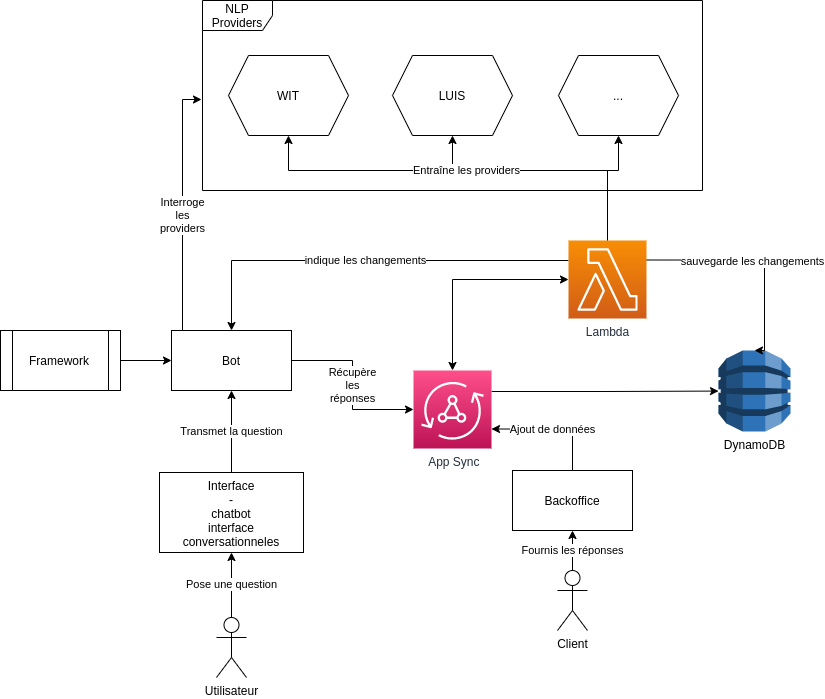
\includegraphics[width=0.9\textwidth]{pictures/kmb_univers.png}
	\caption{Relation entre les différents projets de KMB Labs}
\end{figure}

\section{Technologies}

Outre les services d'AWS, GraphQL et \textit{Serverless}, les interfaces sont réalisées avec le framework React.

React est un framework en perpétuelle évolution permettant de réaliser des interfaces via un système de composant. Chaque élément est donc coder sous forme de fonction utilisant le JSX pour mettre en place l'HTML.

Le JSX, en plus de pouvoir utiliser les balises HTML, permet d'utiliser d'autres composants comme s'ils étaient des balises HTML.

En plus de React, Redux est utilisé dans toutes les interfaces. Redux est un framework connu pour la gestion de \textit{store}, et pour le cas de React un conteneur à état commun à toutes l'application.

En effet, les composants React fonctionnent via une gestion d'états. Chaque changement d'état peu provoquer des changements dans l'interface en mettant à jour le rendu des composants. Redux nous permet de stocker des états que plusieurs composants peuvent utiliser de façon à synchroniser les composants utilisant une donnée commune lorsque celle-ci change.

\chapter{Projets}

Lors de ce stage, plusieurs projets m'ont été confiés. Dans cette partie je détaillerai mes différentes interventions. J'y détaillerai l'objectif du projet ainsi que les différentes tâches qui m'ont été confiées.

\section{Les templates}

Le premier projet auquel j'ai participé, afin de me faire à l'agencement du Backoffice et de comprendre le fonctionnement des différents éléments qui le composent, avait pour objectif de paramétrer plus rapidement les projets.

Les projets, associé aux clients, doivent être lié à des modèles d'apprentissage pour permettre la compréhension d'un domaine. Faisons la comparaison entre l'immobilier et les ressources humaines.

Chaque projet de client est lié à ce qu'on appelle une ou plusieurs catégories. Les catégories regroupent les intentions et sont liées à un \textit{provider}.

Dans l'immobilier, le chatbot doit pouvoir comprendre les intentions liées loyer, prix d'achat et de vente, surface, etc\dots De l'autre côté, un chatbot lié aux ressources humaines devra comprendre les intentions liés aux horaires de travail, au salaire, etc\dots En plus des intentions spécifiques au domaine du chatbot vient s'ajouter des intentions plus générales comme les formules de politesse pour saluer l'utilisateur, réponde à ses remerciements et plus encore.

On retrouve alors des catégories comme l'immobilier, le recrutement, les phrases de politesse, etc...

\begin{problem}
Pour associer un modèle de compréhension à un chatbot, une personne de chez KMB Labs devaient jusqu'alors sélectionner manuellement dans les paramètres du projet ledit modèle.
\end{problem}

\begin{quote}
N.B: ce projet est très diversifié dans sa manière de s'intégrer à l'existant, nous verrons que celui-ci touche à beaucoup d'aspect différents du Backoffice.
\end{quote}

\newpage
\subsection{Objectif}

L'objectif d'ajouter des templates étaient de pouvoir facilement associer plusieurs modèle à un projet en sélectionnant un template. Pour se faire, deux points sont à prendre en compte :
\begin{itemize}
	\item la création du template
	\item l'association à un projet
\end{itemize}

\subsubsection{La création de template}

Pour créer différents éléments du Backoffice (utilisateur, projets, intention) un admin ouvre ce que l'on appelle une \textit{popin}\footnote{interface pouvant s'afficher par dessus le reste de l'application web} en utilisant le bouton correspondant dans les paramètres globaux.

Pour les templates, le même principe a été utilisé. Pour créer un template il faut donc ouvrir la \textit{popin} ce qui ouvre l'interface suivante :

\begin{figure}[!ht]
\centering
	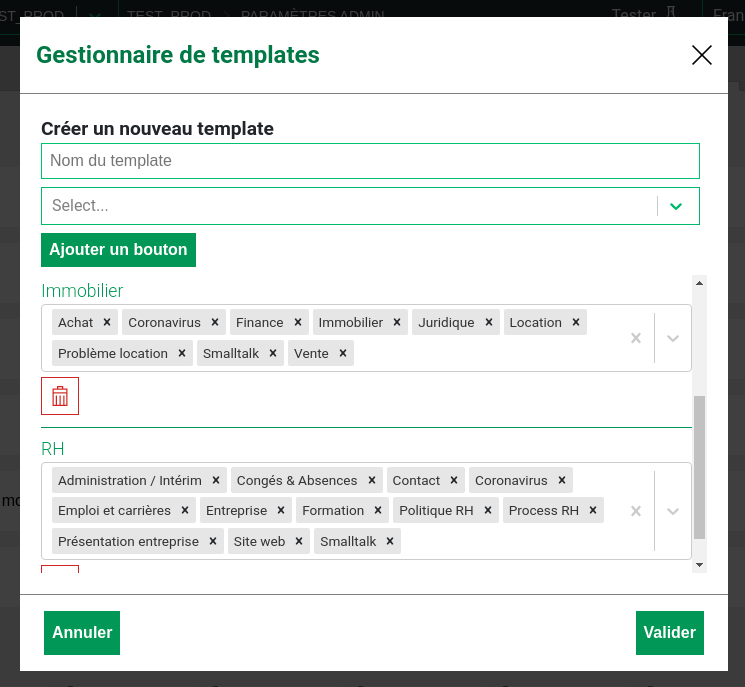
\includegraphics[width=0.75\textwidth]{pictures/popin_create_templates.png}
\end{figure}

L'objectif ici était donc d'ajouter une nouvelle \textit{popin} à l'interface en utilisant l'existant. React étant orienté composant, il est très facile de réutiliser l'existant : le squelette de la fenêtre était déjà réalisé, il ne me restait plus qu'à comprendre comment une \textit{popin} était affichée.

En effet la gestion de celle-ci passe par un \textit{store} Redux\footnote{\href{https://redux.js.org}{\og\textit{A Predictable State Container for JS Apps}\fg{} \textbf{Vu sur redux.js.org} }}. Le gestionnaire des \textit{popins} est toujours affiché, cependant une \textit{popin} n'est affichée seulement si son identifiant est présent dans le store.

Une fois le composant permettant de créer un template intégré à l'interface, il a fallu le relier à la base de donnée. Pour ce premier projet, le schéma de l'API ainsi que la mutation permettant de modifier la base de données ont été réalisée par mon maître de stage, Paul Leménager. De mon côté, il ne me restait plus qu'à les utiliser en gardant en tête la structure d'une requête GraphQL.

\subsubsection{L'association à un projet}

Associer un template à un projet à soulever des questions :
\begin{itemize}
	\item devons nous garder les valeurs existantes ?
	\item le template doit-il être associé par un identifiant au projet ?
\end{itemize}

Pour répondre à la première question, il a fallu dans un premier temps définir les templates qui seront disponibles, avec la liste des catégories d'intentions qui leur seront liées. Puis voir si cela concorde avec les projets existants. Il y a quasiment toujours au moins une catégorie qui n'est pas dans le template qui est utilisée dans chacun des projets. De fait, nous devions garder les valeurs existantes, et toujours pouvoir ajouter une catégorie d'intentions sans pour autant ajouter un template.

Pour le second point, la question a été répondue assez aisément. Même si les templates étaient stockés dans la base de données, associer l'identifiant d'un ou de plusieurs templates à un projet aurait demandé des modifications du schéma de l'API, des lambdas concernées et de créer les liaisons nécessaires pour récupérer les catégories associer au templates pour les ajouter à celles existantes du projet. Nous avons donc pris la décision de faire au plus simple : ajouter aux catégories du projets les catégories du templates, en excluant les doublons éventuels.

Sur le plan de l'interface, une simple liste déroulante permettant de sélectionner un ou plusieurs templates a été ajouté parmi les différents paramètres pré-existant (Voir figure \ref{fig:parameters}).

\begin{figure}[!ht]
	\centering
	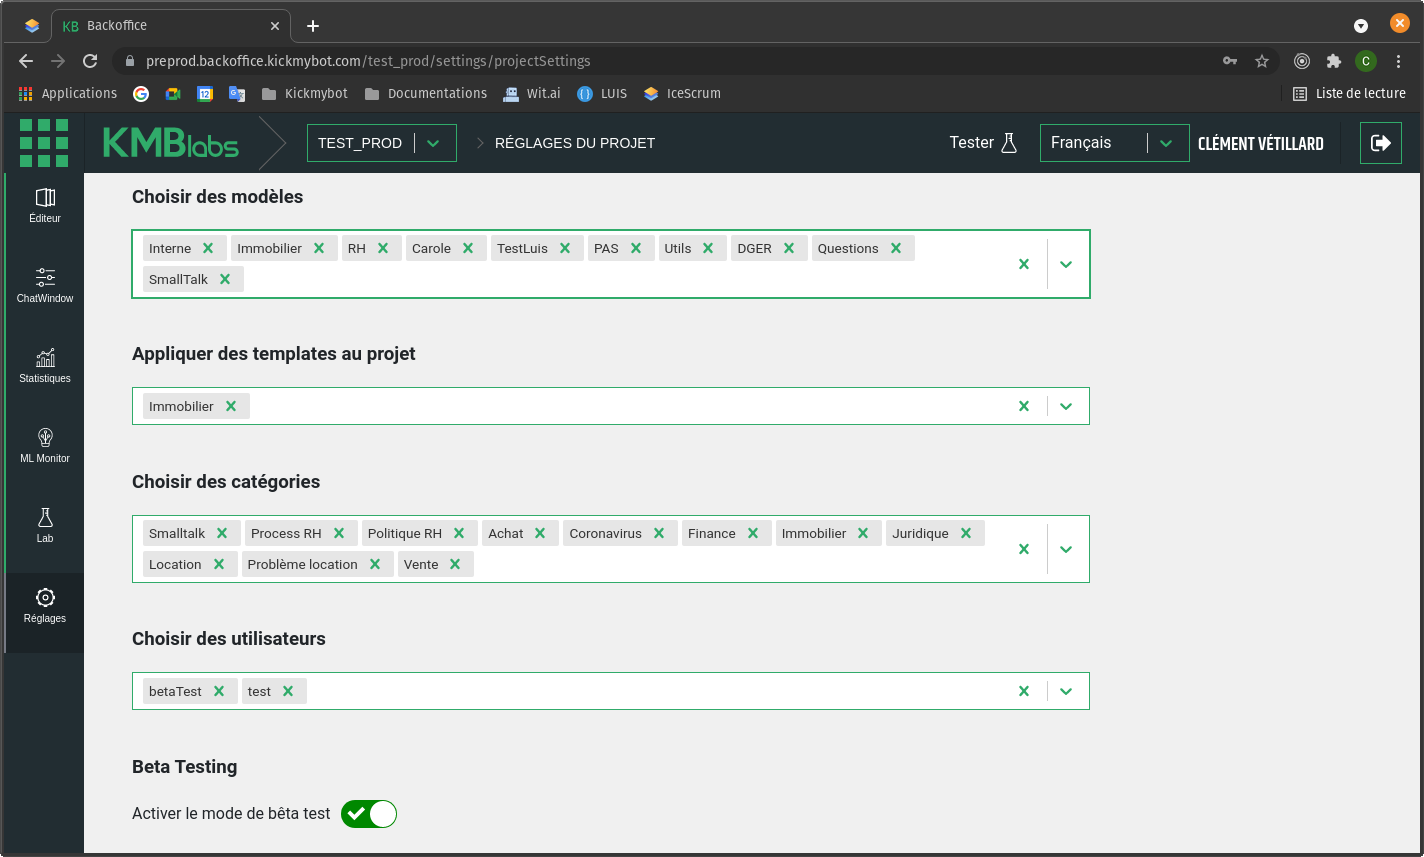
\includegraphics[width=0.9\textwidth]{pictures/template_selector.png}
	\caption{Page de paramétrage d'un projet}
	\label{fig:parameters}
\end{figure}

\begin{result}
	La sélection de templates est gérée dynamiquement en fonction des catégories sélectionnées. De fait, si l'on ajoute un template, on étend la liste des catégories actuelle du projet de façon à reproduire le comportement de l'utilisateur.

	Ainsi, si on ajoute ou supprime une catégorie, la liste des templates est mise à jour en fonction des changements, sans que la base de données n'ait été mise à jour pour intégrer les templates aux projets.
\end{result}

\begin{info}
	Ce premier projet m'a permis d'appréhender les différents concepts qui seront ré-utilisés dans les autres projets liés au Backoffice:
	\begin{itemize}
		\item le store Redux
		\item les \textit{functional component} en React
		\item les \textit{query} et \textit{mutation} GraphQL
		\item les \textit{PopIn}
	\end{itemize}

	Mais aussi les différentes notions propre au domaine de l'entreprise :
	\begin{itemize}
		\item les intentions
		\item les catégories
		\item les projets
	\end{itemize}
\end{info}

\begin{figure}[!ht]
	\centering
	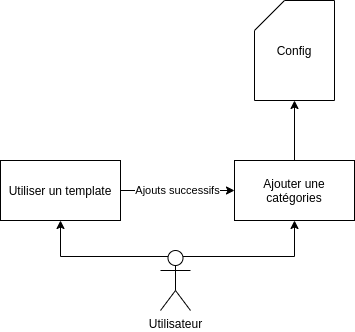
\includegraphics[width=0.9\textwidth]{pictures/diag_template}
	\caption{Schéma fonctionnel du système de template (coloré en vert)}
\end{figure}

\newpage
\section{ML Monitor}

ML Monitor est un outil visant à tester et entraîner les services NLP utilisés. Il est l'aboutissement de réflexion qui ont vu se succéder deux versions \textit{standalone}\footnote{L'outil se trouvait alors sur une application web externe au Backoffice}. J'ai eu la chance lors de ce stage de participer à l'intégration de cette outil au sein même du Backoffice.

Cette intégration a permis de gérer d'une nouvelle manière l'entraînement ainsi que de tester (Voir figures ci-dessous) des modèles de \textit{machine learning}. 

\begin{figure}[!ht]
	\centering
	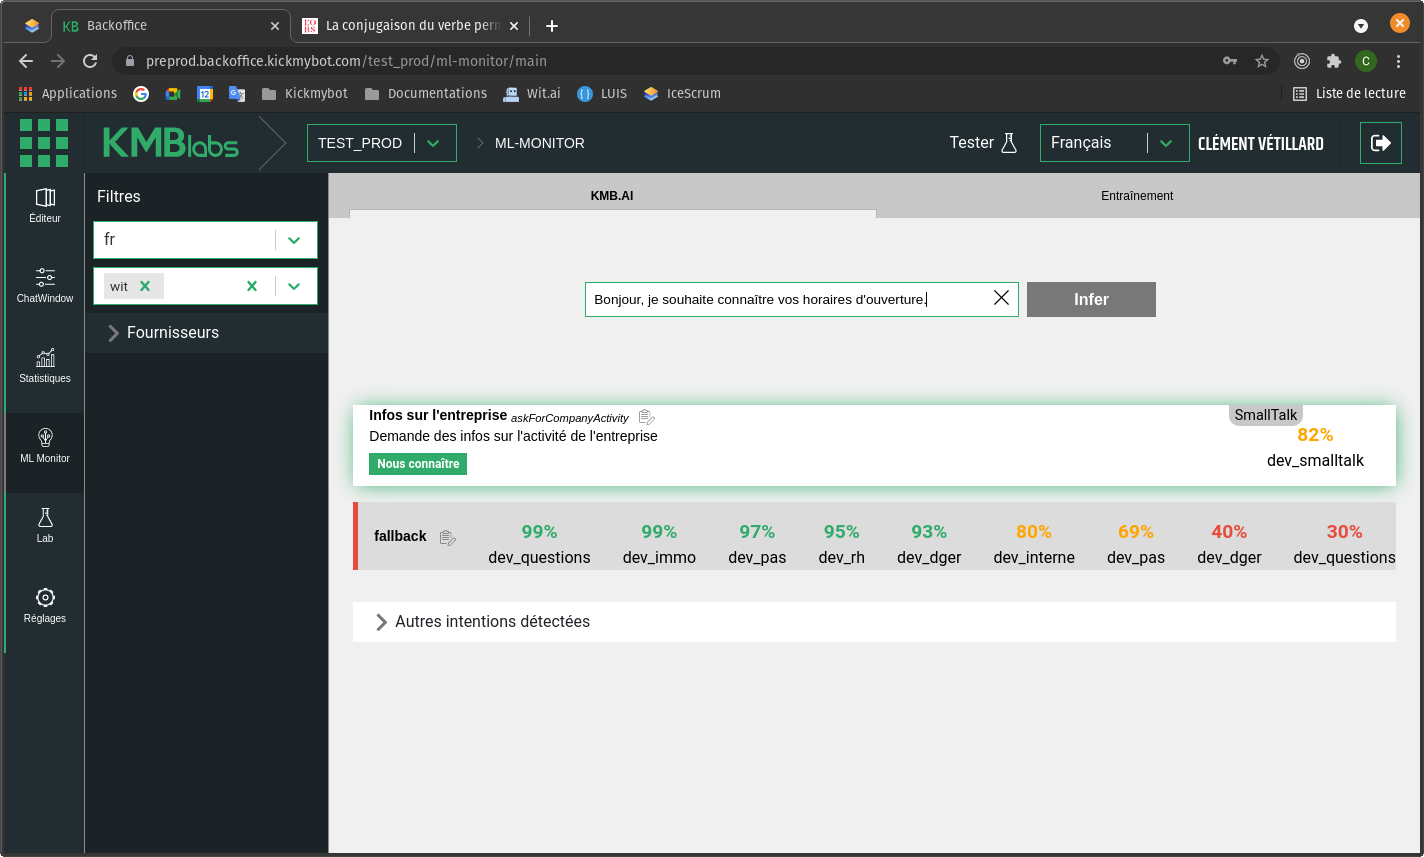
\includegraphics[width=0.7\textwidth]{pictures/mlmonitor_test.png}
	\caption{Page de test de ML Monitor}
	\label{fig:mlmonitor_test}
\end{figure}

\begin{figure}[!ht]
	\centering
	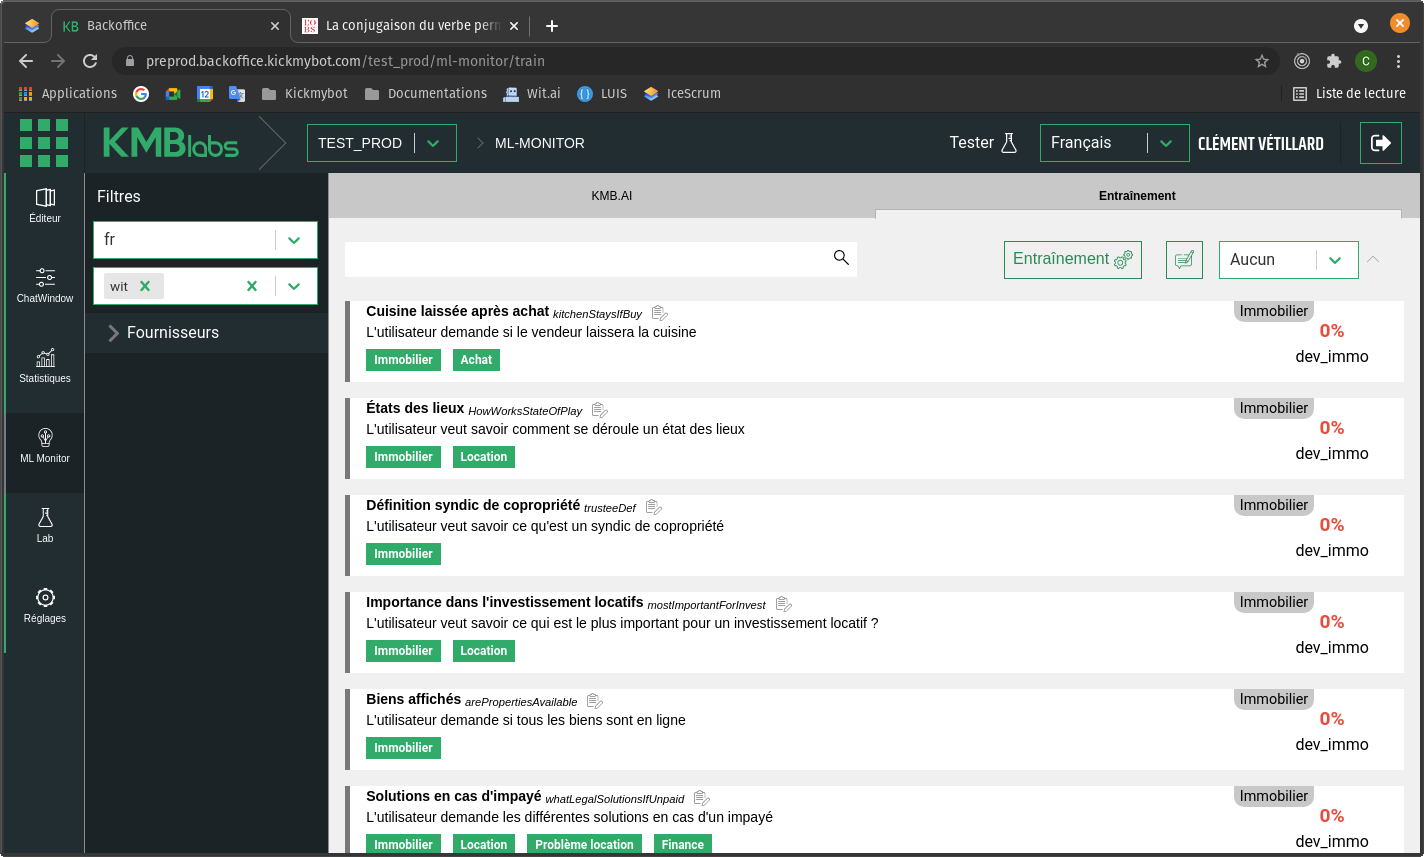
\includegraphics[width=0.7\textwidth]{pictures/mlmonitor_intentions.png}
	\caption{Page listant les intentions de ML Monitor}
	\label{fig:mlmonitor_intentions}
\end{figure}

\begin{figure}[!ht]
	\centering
	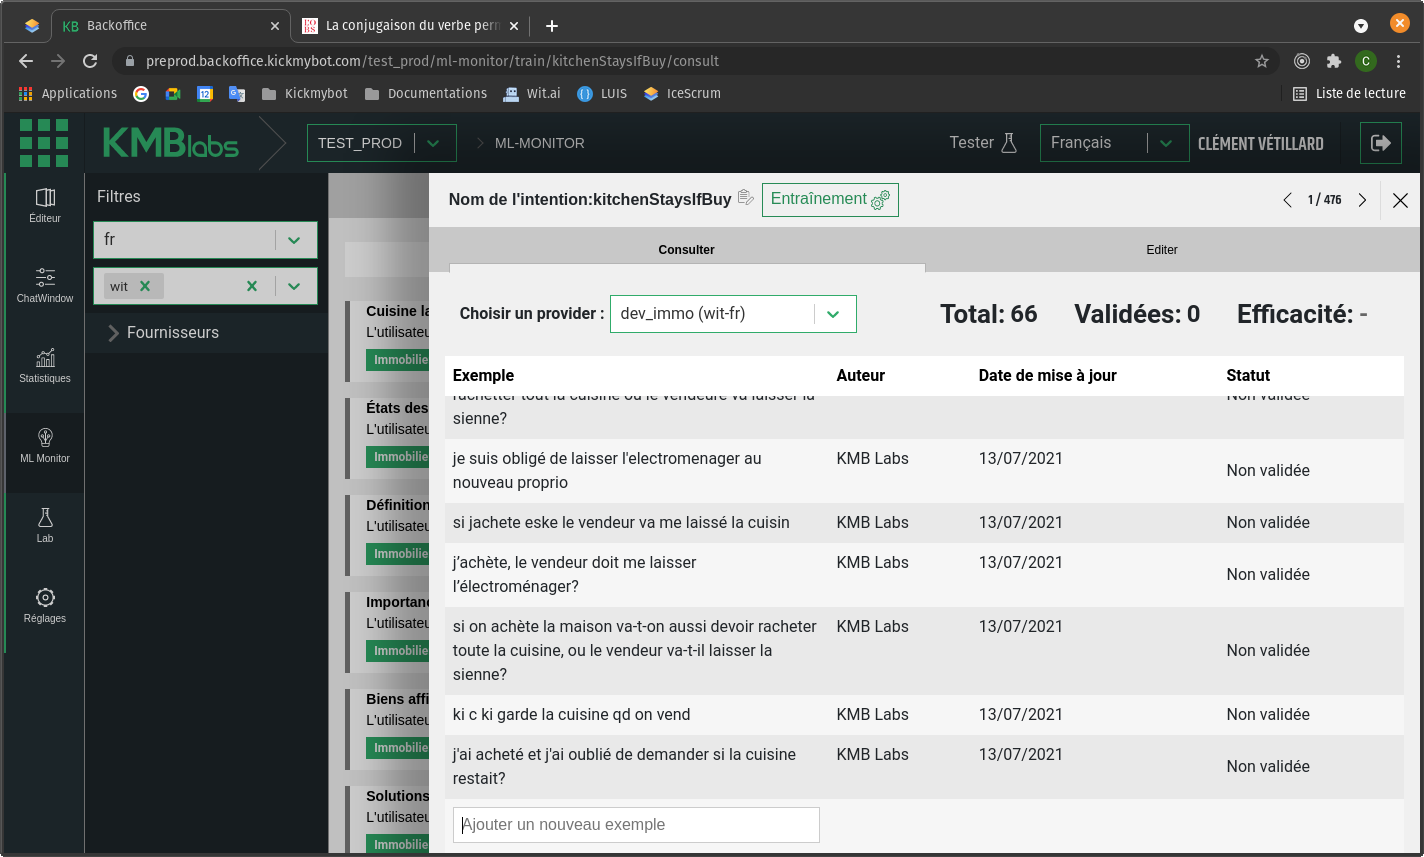
\includegraphics[width=0.9\textwidth]{pictures/mlmonitor_training.png}
	\caption{Page d'entraînement de ML Monitor}
	\label{fig:mlmonitor_training}
\end{figure}
\newpage
Une nouvelle API a été mise en place permettant d'unifier les interactions avec plusieurs fournisseurs NLP.

Actuellement, deux fournisseurs sont utilisés : WIT et Luis (Microsoft). En utilisant cette interface entre NLP et le Backoffice, il est possible d'interagir avec les modèles de chaque fournisseur.

Cette solution permet d'avoir un fournisseur de secours dans le cas où le fournisseur principal ne serait plus disponible.

\begin{figure}[!ht]
	\centering
	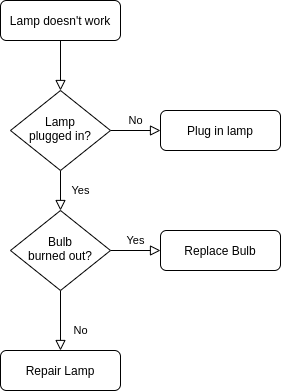
\includegraphics[width=0.7\textwidth]{pictures/diagram_mlmonitor.png}
	\caption{Schéma fonctionnel de ML Monitor}
\end{figure}

\begin{info}
	Ce projet étant une nouvelle partie du Backoffice, j'ai pu participer à l'élaboration de l'interface ainsi que la partie concernée de l'API. J'ai donc pu découvrir les technologies suivantes :
	\begin{itemize}
		\item AppSync (service AWS pour gérer une API GraphQL)
		\item Lambda (service AWS associer une fonction Node.JS à un \textit{endpoint})
		\item DynamoDB et ses requêtes en VTL
		\item CloudWatch (service AWS permettant de surveiller les différents services)
		\item Serverless (permet de gérer l'architecture AWS via des fichiers YAML)
	\end{itemize}
\end{info}

\subsection{Gestion des fournisseurs NLP}

Un des points auxquels j'ai pu participer est la gestion de multiple fournisseurs NLP\footnote{Mentionné "provider" ci-après.} sur l'interface.

En effet, même si l'API permet d'utiliser plusieurs providers de façon simultanée, il est nécessaire de pouvoir visualiser les données d'un seul en particulier afin de s'assurer de son fonctionnement.

La mise en place de cette fonctionnalité dans l'interface a tout d'abord nécessité une nouvelle lambda qui sera ensuite liée au schéma GraphQL. Chaque catégorie d'intentions est liées à au moins un provider pour entraîner un modèle d'apprentissage avec des données traitant un thème commun (\textit{E.G: salutation}).

La lambda, qui se présente sous la forme d'une fonction Node.JS dans notre cas\footnote{Les Lambda AWS supportent de nombreux langages connus comme Node.JS, Python, Java\dots}, se charge donc de récupérer toutes les catégories liées au projet courant afin d'extraire l'ensemble des providers utilisés.

Une fois fait, le schéma GraphQL de l'API a dû être mis à jour avec la nouvelle \textit{query}, et lier la source de données de la \textit{query getProviders} à la lambda en utilisant Serverless. Une fois la connexion entre l'\textit{endpoint} et la \textit{lambda} réalisée, chaque demande de cette donnée sera redirigée vers la nouvelle lambda qui se chargera de récupérer et traiter les informations des catégories pour en extraire la liste des \textit{providers}.

\subsection{L'entraînement des modèles}

Le second point qui a été ma principale participation est l'ajout de l'interface permettant d'entrainer le modèle lié à une intention. L'objectif de cette interface est de pouvoir entrainer un modèle avec plusieurs phrases.

De cette façon, les phrases d'entraînements peuvent être rédigées au préalable, via un tableur par exemple, et une fois validée par les personnes compétentes, peuvent être importées dans le modèle via un simple copier/coller.

La mise en place de cette solution a nécessité quelques ajustements, notamment au niveau du schéma de l'API afin de prendre en charge une liste de phrases et non plus une simple phrase, afin de limiter les appels à l'API, puis de modifier la \textit{lambda} associée en conséquence.

La lambda a pour objectif de :
\begin{enumerate}
	\item mettre à jour la base de données DynamoDB (qui fait foi dans le cas d'un entraînement de l'intégralité du modèle)
	\item ajouter les phrases dans chaque provider et lancer la procédure d'inférence afin que les changements soit pris en compte le plus rapidement possible
\end{enumerate}

\section{Éditeur WYSIWYG}

L'éditeur WYSIWYG\footnote{What You See Is What You Get} est un ajout que j'ai pu réaliser, avec l'intégration de Draft.js\footnote{Facebook opensource} et de différents plugins permettant ainsi d'obtenir un éditeur plus agréable pour l'utilisateur.

\begin{figure}[!ht]
	\centering
	
\includegraphics[scale=0.75]{pictures/wysiwyg.png}
	\caption{Aperçu de l'éditeur tel qu'il est présent dans le Backoffice}
\end{figure}

Cette éditeur a été utilisé en remplacement d'un éditeur plus basic où le style n'était pas interprété. Le format utilisé nativement par l'éditeur est de l'HTML, cependant un système de conversion a été mis en place afin de correspondre aux formats utilisés dans les fenêtres de discussion de \textit{chatbot}.

\begin{info}
	L'éditeur est une partie plus accessoire mais qui a vu quelques complications dû à la gestion de l'état de l'éditeur Draft.JS.

	Celui-ci est assez complexe, et comme tous les composants React, doit être prédictible. De fait, chaque modification manuelle implique de reconstruire l'état en utilisant les valeurs précédentes pour garder un éditeur stable (sélection, position du curseur, style, etc\dots).

	De plus, la gestion des tags personnalisés en lieu et place des balises HTML a nécessité la mise en place d'expression régulière permettant de sélectionner les tags pour l'import dans l'éditeur, puis des balises HTML pour l'export.
\end{info}

\section{ChatWindow}

La section ChatWindow du Backoffice est la dernière partie de cette application sur laquelle j'ai particpé durant mon stage. Cette dernière consiste à paramétrer de façon visuel quelques aspects de la fenêtre de discussion des chatbots.

Entre autres, cette section va permettre de configurer les \textit{Fast Action} qui prennent la forme de bouton au dessus de l'icône du \textit{chatbot} comme le montre l'image suivante.

\begin{figure}[!ht]
	\centering
	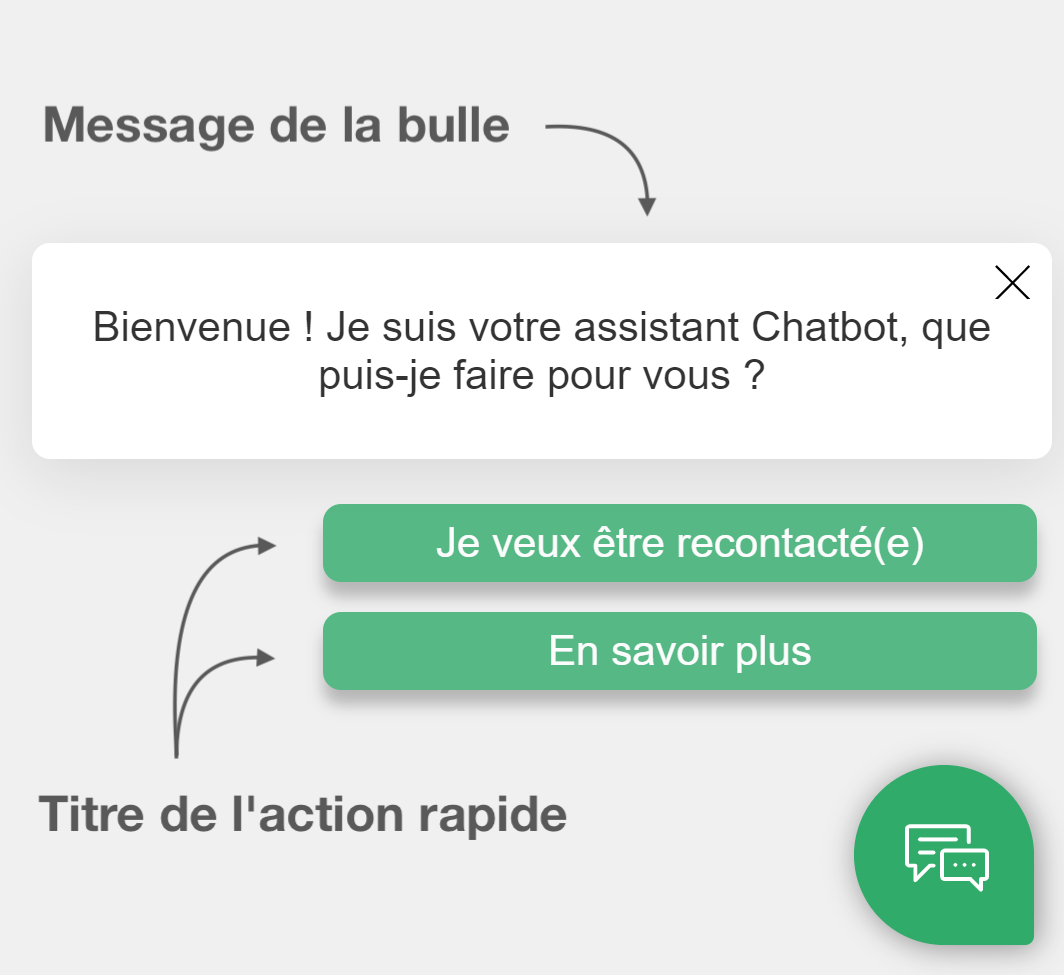
\includegraphics[width=5.9cm]{pictures/fa.png}
	\caption{Image issue du Backoffice illustrant la fenêtre du \textit{chatbot}}
\end{figure}

L'avantage des \textit{Fast Actions} est que le \textit{chatbot} n'utilise pas les \textit{providers} afin d'obtenir les résultats, elles sont directement reliées à une intentions ou bien une réponse définie. De cette façon, l'utilisateur du chatbot peut avoir une réponse instantannée en utilisant ces boutons.

Afin de donner une certaine polyvalence aux \textit{Fast Actions}, celle-ci sont regroupées par page. Chaque page possède une configuration qui lui est propre et qui est configurage via l'interface ChatWindow. On peut donc spécifier une URL d'activation, qui peut être une URL complète, la base d'une URL ou bien une expression régulière.

\subsection*{Création des réponses}

La mise en place de ChatWindow dans le Backoffice a permis de réutiliser les éléments déjà en place et d'enrichir les réponses possibles. Avant l'apparition de cette section, les actions rapides pouvaient être liées à une intention, une réponse texte ou bien à une redirection vers une URL donnée.

Bien que ces trois éléments étaient déjà présent lorsque la configuration du \textit{chatbot} ne se faisait que via l'édition d'un fichier JSON, l'interface permet de visualiser les éléments de réponse :
\begin{itemize}
	\item l'intention sélectionnée est affichée via son nom au lieu de son identifiant
	\item une réponse texte est affichées avec le style interprété (éditeur WYSIWYG)
	\subitem - ces réponses sont sauvegardées de la même manière que celles liées à une intention, de cette façon plusieurs réponses successives peuvent être ajouter et des médias peuvent y être joints.
	\item la redirection URL est validée avant sauvegarde (expression régulière)
\end{itemize}

\section{Interface conversationnelle}

L'interface conversationnelle se présente sous la forme d'une page entière (à contrario du \textit{chatbot}). Utilisée comme moteur de recherche, cette interface peut tout de même répondre aux questions liées à des intentions.

La partie recherche est augmentée par le NLP ce qui permet de détecter les filtres possibles dans la recherche de l'utilisateur (localisation, salaire, loyer, surface, etc\dots). Cette solution rend l'expérience de recherche plus simple pour l'utilisateur, permettant ainsi d'effectuer des recherches en utilisant formulant une demande.

La particularité de l'interface conversationnelle est qu'un seul projet gère les intégrations de plusieurs clients. En effet, la réalisation de ce projet est orientée \textit{config-first}. C'est à dire que chaque élément spécifique au client (nommage, pages disponibles, filtres disponible, etc\dots) est entièrement géré dans un dossier de configuration qui lui ait propre. Par la suite, l'application du client peut-être générée grâce à Webpack qui nous permet de sélectionner la bonne configuration facilement avec les variables d'environnement.

\subsection{La page d'aiguillage}

La page d'aiguillage est un nouvel ajout nécessaire pour l'intégration d'un client. Celle-ci permet de récupérer le résultat de plusieurs flux de données, selon une recherche donnée, et de présenter les dix premiers résultats.

Avant la création de cette page, plusieurs flux pouvaient être géré par l'interface mais pas de façon simultanée. Une recherche était liée à un flux unique.

Cette particularité a demandé la modification d'une partie des composants avec l'ajout d'une page entière.

\begin{info}
	Ma participation sur ce projet n'a pas été importante. Cependant, l'approche \textit{config-first} a été une nouveautée avec laquelle j'ai apprécier travailler malgré les difficultées rencontrées. J'ai pu enrichir les composants globaux ainsi que ceux spécifiques à un projet.

	La principale difficulté ici est de s'intégrer à l'existant : comprendre le fonctionnement des configurations, la manière de récupérer la configuration selon la page courante, etc\dots
\end{info}

\section{Optimisation Chat-Window}

Le \textit{Chat-Window}\footnote{Interface du \textit{chatbot}.} est le produit le plus commercialisé par KMB Labs. Au fur et à mesure des ajouts le poids du script JavaScript permettant son exécution a augmenté et est devenue problématique.

En effet, le temps de chargement du script, pourtant décalé vis à vis du chargement du site hôte, provoque des ralentissements pour l'utilisateur. Ce ralentissement dépend de la machine utilisée ainsi que du débit internet, cependant il existe toujours\footnote{Notamment via les tests Lighthouse}.

Pour palier ce problème, j'ai réalisé des recherches quant aux possibilités à notre disposition pour remédier à ce problème.

\begin{problem}
	Comment diminuer le poids du \textit{bundle} tout en gardant l'intégralité des fonctionnalités disponibles ?
\end{problem}

\subsection{Webpack - Chunks}

React embarque l'outil Webpack afin de compresser tout un projet web dans un seul fichier JavaScript.

Diverses plugins et options permettent de découper les projets afin de séparer les ressources. Globablement, l'utilisation des \textit{chunks} est souvent utilisée pour séparer les \textit{assets} ainsi que les modules issue de Node.js et de NPM dans des chunks à part. Ceux-ci étant rarement modifiés, les chunk resteront en cache dans le navigateur et ne seront chargés qu'une seule fois.

Cette solution n'empêche pas les ralentissement au premier chargement, mais peut grandement accélérer les chargements ultérieurs. Or, dans le cas de \textit{chatbot}, l'utilisateur n'est pas forcément amené à utiliser régulièrement l'assistant. J'ai donc cherché une autre possibilité permettant de charger les modules uniquement au moment de leur première utilisation.

\begin{figure}[!ht]
	\centering
	
\includegraphics[width=\textwidth]{pictures/webpack_chunks.png}
	\caption{Exemple de répartition manuelle des chunks}
\end{figure}

\newpage
\subsection{Les imports dynamiques}

L'ECMAScript 2020 voit apparaître la possibilité d'importer dynamiquement une dépendance via la fonction \textbf{import()}. Cette fonction va retourner une \textit{Promise} à l'import d'un module.

En rencontrant cette notation lors du processus de \og\textit{bundling}\fg{}, Webpack va autommatiquement commencer à découper le code sous-jacent en chunks indépendant tout en regroupant les dépendances communes à plusieurs chunk.

La grande force de cette approche est que React propose depuis la version 17 les outils nécessaires à son utilisation. Chaque composant à importer dynamiquement peut être charger via la fonction \textit{lazy} de React. Cette fonction prend en paramètre un \textit{callback} utilisant le fonction d'import citée plus haut.

De cette façon, React fourni les outils pour :
\begin{itemize}
	\item importer de façon asynchrone un composant et ses dépendances
	\item gérer le cas où un composant n'est pas encore charger (via un composant issu de React (\textit{Suspense}) encadrant les composants asynchrone)
\end{itemize}

Dans le diagrame ci-dessous, un exemple de chunks dynamiques regroupés par couleur.

\begin{figure}[!ht]
	\centering
	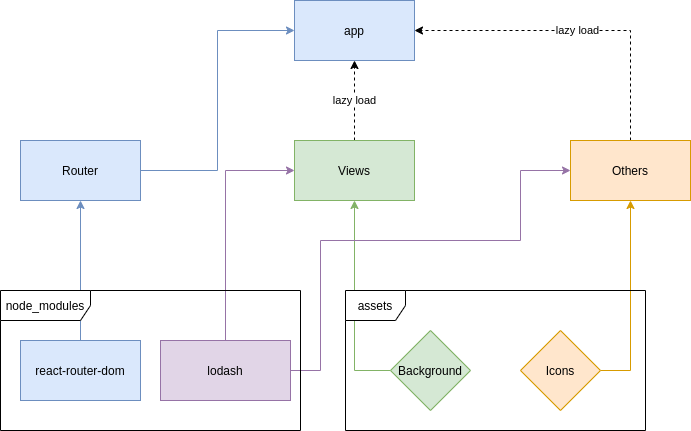
\includegraphics[width=\textwidth]{pictures/dynamics_imports.png}
	\caption{Example de répartition dynamique des chunks}
\end{figure}

\begin{info}
	La première étape pour la réalisation de cette optimisation est de mettre à jour toutes les dépendances nécessaires avant de pouvoir commencer à mettre à jour le code et utiliser ces nouveaux outils.

	Ensuite, la conversion des composants basés sur le système de \textit{class} vers les \textit{functional components} s'est avéré obligatoire afin d'utiliser les outils fournis par React.

	Une fois fait, les modules les plus lourd ont été ciblé en premier lieu afin d'obtenir un résultat probant le plus rapidement possible afin d'alléger le poids du build pour tous les clients utilisant le \textit{chatbot}.
\end{info}

\begin{result}
	Cette approche a été choisie car permet un découpage plus précis du code permettant d'avoir un chargement initial comportant uniquement les éléments vitals à l'affichage de la bulle du \textit{chatbot} sans charger tous les comportements de la fenêtre.

	À titre de comparaison, avant la mise en place sur quelques composants, le chargement initial comportait un téléchargement d'un fichier d'environs 700ko. Avec l'utilisation du \textit{lazy loading}, le chargement initial était descendu à 400ko en ayant transformé que quelques composants.
\end{result}

\chapter{Conslusion}

Lors de ce stage, j'ai pu participer au développement de solutions basées sur des technologies du traitement du langage naturel. KMB Labs est une start-up composée d'une petite équipe de développeurs utilisant des technologies en vogues (aussi bien pour les interfaces utilisateurs que pour la partie serveur).

Ayant participer à de nombreux ajouts de fonctionnalités, j'ai eu l'occasion d'appréhender les enjeux d'un produit commercialisé, avec parfois des problèmes non répertoriés lors des tests qui sont remontés par des clients ; les complications dû à des refontes d'une partie du code. Mais aussi le travail en équipe avec chaque interlocuteur ayant une spécialité, aussi bien en terme de technologies que de programmation ; où l'échange encouragé malgré la pandémie par des outils adaptés (Slack et Google Meet notamment) permet de garder un contact humain.

Ce stage a été pour moi l'occasion de découvrir un monde professionnel dynamique évoluant dans mon domaine d'étude. Où la théorie fait place à de vraies solutions qui ont sû faire leur place sur le marché.

\end{document}
